\documentclass{article}
\title{ECE 341 -- Homework 2}
\usepackage{graphicx}
\usepackage[margin=1in]{geometry}
\usepackage{float}
\usepackage{pdfpages}
\usepackage{fancyhdr}
\usepackage{enumitem}
\usepackage{pdfpages}
\usepackage{amsmath}
\usepackage{amssymb}
\pagestyle{fancy}
\fancyhf{}
\fancyhead[L]{Gianni Avilan-Losee}
\fancyhead[C]{ECE 341}
\fancyhead[R]{Homework 2}
\fancyfoot[C]{\thepage}
\usepackage{microtype}
\usepackage{textcomp, gensymb}
\author{Gianni Avilan-Losee}
\begin{document}

\includepdf{homework-2_cover-page.pdf}
\begin{enumerate}[label=\thesubsubsection]
\setcounter{section}{2}
\setcounter{subsection}{2}
\setcounter{subsubsection}{1}
\item
\begin{enumerate}[label=(\alph*), start=2]
	\item Given the system described by 
		\[
		\ddot{y}(t) + 2\dot{y}(t) + 5y(t) = \ddot{x}(t) - 5x(t),
		\]
		with initial conditions
		\begin{align*}
		 &y_{\mathrm{zir}}(0) = 4 \\
		 &\dot{y}_{\mathrm{zir}}(0) = -1,
		\end{align*}
		begin by setting \(P(D)x(t)\) to zero to find the zero-input response, \(y_{\mathrm{zir}}(t) = c_1e^{\lambda_1 t} + c_2e^{\lambda_2 t}\).

		To find \(\lambda_1\) and \(\lambda_2\), solve the characteristic equation \(\lambda^2 + 2\lambda + 5=0 \), which returns two complex values, 
		\[
			\lambda_1 = -1+j2, \ \lambda_2 = -1-j2.
		\]
		We can pick two way to solve for \(c_1\) and \(c_2\): we can keep the equation in complex form and solve for the constants, or we can assume that the given system is real and therefore must have a real ZIR, which will allow us to solve for the constants \(c_1\) and \(c_2\) more easily. If assume that the ZIR is real, the \(c_1\) and \(c_2\) must be conjugates, expressed as 
		\begin{align*}
			& c_1 = \frac{c}{2}e^{j\theta} \\
			& c_2 = \frac{c}{2}e^{-j\theta}.
		\end{align*}
		Substituting these new constants into our expression for \(y_{\mathrm{zir}}\), 
		\[
			y_{\mathrm{zir}}(t) = \frac{c}{2}e^{j\theta}e^{(-1+j2)t} + \frac{c}{2}e^{-j\theta}e^{(-1-j2)t} = \frac{c}{2}[e^{-t}e^{j(2t+\theta)} + e^{-t}e^{j(-2t-\theta)}]. 
		\]
		Simplifying using Euler's formula, \(e^{jx} = \cos{(x)} + j\sin{(x)}\),
		\[
			y_{\mathrm{zir}}(t) = \frac{ce^{-t}}{2}[\cos{(2t+\theta)} + j\sin{(2t+\theta)} + \cos{(-2t-\theta)} + j\sin{(-2t-\theta)}.]
		\]
		Since \(\cos{(-x)} = \cos{(x)}\) and \(\sin{(-x)} = -\sin{(x)}\), this reduces to 
		\[
		\frac{ce^{-t}}{2}(2\cos{(2t+\theta)}) = ce^{-t}\cos{(2t+\theta)}.
		\]
		Now, we can easily solve for \(c\) and \(\theta\) in the real domain by setting \(t=0\) for \(y_{\mathrm{zir}}(t)\) and \(\dot{y}_{\mathrm{zir}}(t)\), 
		\begin{align*}
		 & y_{\mathrm{zir}}(t) = ce^{-t}\cos{(2t+\theta)} \\
		 & \dot{y}_{\mathrm{zir}}(t) = -ce^{-t}\cos{(2t+\theta)} - 2ce^{-t}\sin{(2t+\theta)}.
		\end{align*}
		Setting these expressions equal to the given initial conditions with \(t=0\), 
		\begin{align*}
			&y_{\mathrm{zir}}(0) = c\cos{(\theta)} = 4 \\ 
			&\dot{y}_{\mathrm{zir}}(0) = c\cos{(\theta)} - 2c\sin{(\theta)} = -1.
		\end{align*}
		Solving for \(c\cos{(\theta)}\) and \(c\sin{(\theta)}\) using a system of equations,  
		\begin{align*}
			&\begin{bmatrix}
				1 & 0 \\
        1	& -2
			\end{bmatrix}
			\begin{bmatrix}
				c\cos{(\theta)} \\
				c\sin{(\theta)}
			\end{bmatrix} = 
			\begin{bmatrix}
				4 \\
				-1
			\end{bmatrix} \\ \\
			&\begin{bmatrix}
				1 & 0 & 4 \\
				1 & -2 & -1
			\end{bmatrix}
			\Rightarrow \ 
			\begin{matrix}
				&c\cos{(\theta)} = 4 \\
				&c\sin{(\theta)} = 1.5
			\end{matrix}
		\end{align*}
		Considering both terms as the two coordinates of a complex number, we may solve for \(c\) and \(\theta\) as \(c = \sqrt{4^2 + 1.5^2} = 4.272\) and \(\theta = \tan^{-1}{\frac{1.5}{4}} = 0.359\), we can substitute this back into our solution for \(y_{\mathrm{zir}}(t)\), which gives us the complete ZIR, 
		\[
			y_{\mathrm{zir}}(t) = 4.272e^{-t}\cos{(2t + 0.359)}.
		\]
		Finally, we can convert our values for \(c\) and \(\theta\) back to \(c_1\) and \(c_2\) if we want, as 
		\begin{align*}
			&c_1 = \frac{c}{2}e^{j\theta} = 2.136e^{j0.359} \\
			&c_2 = \frac{c}{2}e^{-j\theta} = 2.136e^{-j0.359}.
		\end{align*}
		Then the equivalent, complex ZIR would be 
		\[
			y_{\mathrm{zir}}(t) = 2.136e^{(-1+j0.359)t} + 2.136e^{(-1-j0.359)t}.
		\]
		As mentioned, both equations are equivalent, and show an oscillatory, decaying response to the inital conditions, which is to be expected given complex-valued characteristic roots.

		See Fig. 1 for a plot of the ZIR.

		\begin{figure}[H]
		  \centering
			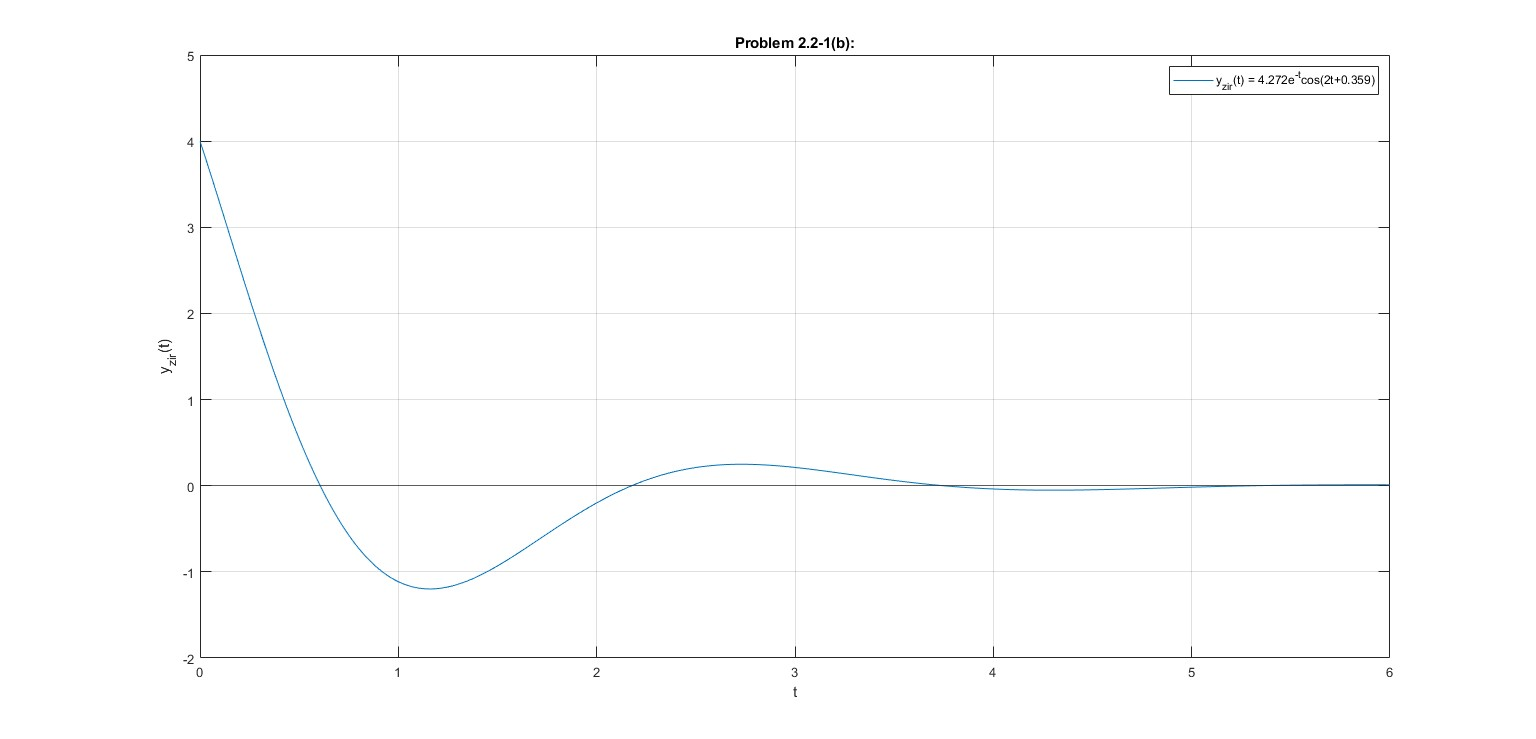
\includegraphics[width=\textwidth]{homework-2_fig-1.jpg}
		  \caption{ZIR response}
		  \label{fig:ZIR 2.2-1(b)}
		\end{figure}
\end{enumerate}
\end{enumerate}
\end{document}
